\addcontentsline{toc}{chapter}{Контрольная работа 1}
\chapter*{Контрольная работа 1}

\addcontentsline{toc}{section}{Вариант 1}
\section*{Вариант 1}

\subsubsection*{1}

\textit{Задание.} В сундуке лежат 10 красных, 6 синих и 4 зелёных пуговицы.
Найдите вероятность того, что две наугад вынутые пуговицы будут разного цвета.

\textit{Решение.}
Опишем пространство элементарных исходов: $ \Omega = \\ = \left\{ \left( x, y \right), \, x, y \in \right.$ красный, синий, зелёный\}\}.
Нужно выбрать две пуговицы из двадцати, поэтому $ \left| \Omega \right| = C_{20}^2$.

Опишем событие $A =$ \{две наугад вынутые пуговицы будут разного цвета\} $= \left\{ \left( x, y \right) in \Omega: \, x \neq y \right\} $.
Выберем сначала одну красную пуговицу --- $C_{10}^1$, а затем --- одну синюю --- $C_6^1$.
По правилу умножения есть $C_{10}^1 \cdot C_6^1$ способов вынуть одну красную и одну синюю пуговицу.
Второй случай: одна из пуговиц красная, другая --- зелёная --- $C_{10}^1 \cdot C_4^1$.
Третий случай: одна из пуговиц синяя, другая --- зелёная --- $C_6^1 \cdot C_4^1$.
По правилу суммы имеем, что $ \left| A \right| = C_{10}^1 \cdot C_6^1 + C_{10}^1 \cdot C_4^1 + C_6^1 \cdot C_4^1$.

Тогда вероятность равна
$$P \left( A \right) =
\frac{ \left| A \right| }{ \left| \Omega \right| } =
\frac{C_{10}^1 \cdot C_6^1 + C_{10}^1 \cdot C_4^1 + C_6^1 \cdot C_4^1}{C_{20}^2}.$$

\subsubsection*{2}

\textit{Задание.} Подбросили 10 игральных кубиков.
Найдите вероятность того, что единица выпала хотя бы на двух кубиках, если известно, что она выпала хотя бы на одном кубике.

\textit{Решение.}
Опишем пространство элементарных событий:
$ \Omega = \\
= \left\{ \left( x_1, x_2, \dotsc, x_{10} \right): \,
x_i \in \left\{1, 2, 3, 4, 5, 6 \right\}, \,
i =
\overline{1, 6} \right\} $.
На каждом кубике может выпасть число от одного до шести (6 вариантов), поэтому $ \left| \Omega \right| = 6^{10}$.

Рассмотрим событие $A =$ \{единица не выпала ни на одном кубике\}.
На каждом кубике может выпасть число от одного до пяти.
Таких вариантов есть $5^{10}$.
Тогда вероятность события $A$ равна
$$P \left( A \right) =
\frac{ \left| A \right| }{ \left| \Omega \right| } =
\frac{5^{10}}{6^{10}}.$$

Тогда событие $ \overline{A} =$ \{единица выпала хотя бы на одном кубике\} имеем вероятность
$$P \left( \overline{A} \right) =
1 - P \left( A \right) =
1 - \frac{5^{10}}{6^{10}}.$$

Рассмотрим событие $B =$ \{единица выпала хотя бы на двух кубиках\}.
Рассмотрим пересечение событий $ \overline{A} \cap B =$ \{единица выпала хотя бы на двух кубиках\} $= B$.
Рассмотрим противоположное событие: $ \overline{B} =$ \{единица выпала ровно на одном кубике\} $
\cup $ \{единица не выпала ни на одном кубике\} $= B_1 \cup A$.
Найдём количество способов выпадения цифр на кубиках, которые ему удовлетворяют.

$B_1 =$ \{единица выпала ровно на одном кубике\}.
Нужно выбрать 1 кубик из десяти, на котором выпала единица --- это $C_{10}^1$.
На остальных десяти кубиках может быть любое число от двух до шести --- $5^9$.
По правилу умножения $ \left| B_1 \right| = C_{10}^1 \cdot 5^9$.
Вероятность этого события равна
$$P \left( B_1 \right) =
\frac{ \left| B_1 \right) }{ \left| \Omega \right| } =
\frac{C_{10}^1 \cdot 5^9}{6^{10}}.$$

Тогда вероятность события $B$ равна
$$P \left( B \right) =
P \left( A \right) + P \left( B_1 \right) =
\frac{5^{10}}{6^{10}} + \frac{C_{10}^1 \cdot 5^9}{6^{10}} =
\frac{5^{10} + C_{10}^1 \cdot 5^9}{6^{10}}.$$

Условная вероятность события $B$ при условии, что событие $ \overline{A}$ произошло, равна
$$P \left( \left. B \right| \overline{A} \right) =
\frac{P \left( \overline{A} \cap B \right)}{P \left( \overline{A} \right) } =
\frac{P \left( B \right)}{P \left( \overline{A} \right) } =
\frac{ \frac{5^{10} + C_{10}^1 \cdot 5^9}{6^{10}}}{1 - \frac{5^{10}}{6^{10}} }.$$

\subsubsection*{3}

\textit{Задание.} Допустим, что в среднем 5 мужчин из 100 и 25 женщин из 10000 являются дальтониками.
Наугад выбранный человек оказался дальтоником.
Какая вероятность того, что это был мужчина?

\textit{Решение.} Рассмотрим событие $A =$ \{наугад быбранный человек оказался дальтоником\}.
Рассмотрим гипотезы: $H_1 =$ \{выбранный человек --- мужчина\}, $H_2 =$ \{выбранный человек --- женщина\}.
Мужчин и женщин в популяции одинаковое количество, поэтому вероятности гипотез равны
$$P \left( H_1 \right) =
\frac{1}{2} =
P \left( H_2 \right).$$
Условные вероятности:
$$P \left( \left. A \right| H_1 \right) =
\frac{5}{100}, \,
P \left( \left. A \right| H_2 \right) =
\frac{25}{10000}.$$
По формуле Байеса
$$P \left( \left. H_1 \right| A \right) =
\frac{P \left( \left. A \right| H_1 \right) P \left( H_1 \right) }{P \left( \left. A \right| H_1 \right) P \left( H_1 \right) +
P \left( \left. A \right| H_2 \right) P \left( H_2 \right) } =
\frac{ \frac{5}{100} \cdot \frac{1}{2} }{ \frac{5}{100} \cdot \frac{1}{2} +  \frac{25}{10000} \cdot \frac{1}{2} }.$$

\subsubsection*{4}

\textit{Задание.} Петя играет в орлянку.
Он начинает игру, имея одну гривну.
Если выпадет орёл, то Петя получает одну гравну, в другом случае --- теряет одну гривну.
Была сиграна 21 игра, после которой Петя остался без денег и без долга.
Найдите вероятность того, что Петя впервые остался без денег именно в последней игре.

\textit{Решение.} На рисунке \ref{fig:14} изображены возможные пути.

\begin{figure}[h!]
  \centering
  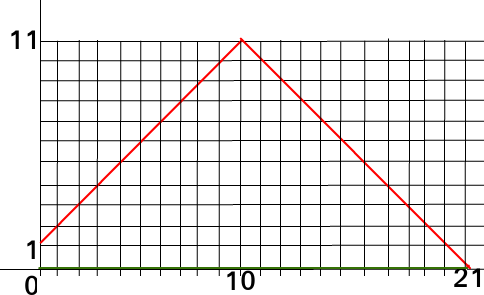
\includegraphics[width=.4\textwidth]{./pictures/t1v1_4.png}
  \caption{Пути}
  \label{fig:14}
\end{figure}

Они ограничиваются красной линией.
Зелёную линию пересекать не можем.
Касаться её можно только в точке $ \left( 21, 0 \right) $.

Перевернём изображение (рис. \ref{fig:1	41}).

\begin{figure}[h!]
  \centering
  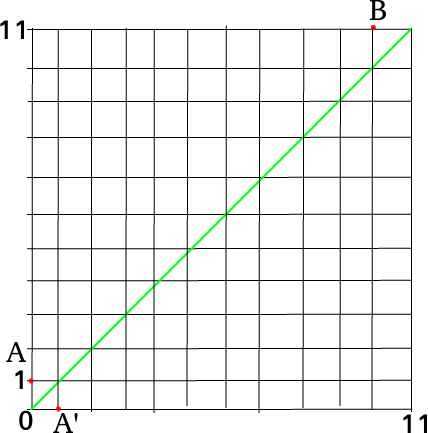
\includegraphics[width=.4\textwidth]{./pictures/t1v1_41.png}
  \caption{Перевёрнутое изображение}
  \label{fig:141}
\end{figure}

Теперь можем ходить направо и вверх.
Всего путей из точки $A$ (начальной) в точку $B$ (конечную) $C_{10+11}^{10} = C_{21}^{10}$.
По методу отражения путей, которые касаются или пересекают диагональ столько, сколько путей из точки $A'$ в точку $B$.
Их $C_{9+11}^9 = C_{20}^9$.
Тогда путей, которые не касаются и не пересекают диагональ $C_{21}^{10} - C_{20}^9$.

А вероятность такого события равна
$$P =
\frac{C_{21}^{10} - C_{20}^9}{C_{21}^{10}}.$$

\subsubsection*{5}

\textit{Задание.} В равнобедренный прямоугольный треугольник с катетами длиной $1$ см наугад бросили точку.
Найдите вероятность того, что расстояние от этой точки до какой-то из вершин треугольника не превышает 0.5 см.

\textit{Решение.} Эта задача на геометрическую вероятность.
Пространство элементарных событий $ \Omega $ --- равнобедренный прямоугольный треугольник с катетами длиной 1.
Его площадь равна
$$S_{ \Omega } =
\frac{1}{2} \cdot 1 \cdot 1 =
\frac{1}{2}.$$
Событие $A =$ \{расстояние от наугад выбранной точки в данном треугольнике до какой-то из его вершин не превышает 0.5\} на рисунке \ref{fig:5} закрашено чёрным цветом.

\begin{figure}[h!]
  \centering
  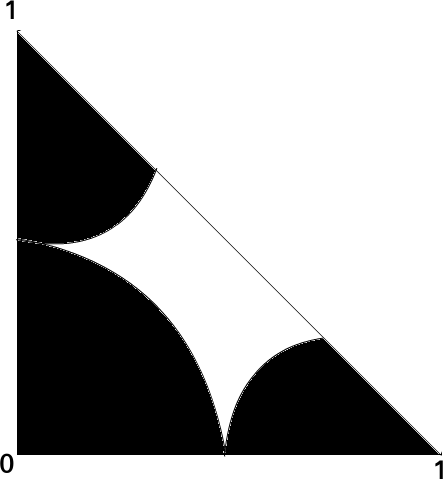
\includegraphics[width=.4\textwidth]{./pictures/t1v1_5.png}
  \caption{Пространство элементарных событий $ \Omega $ и событие $A$}
  \label{fig:5}
\end{figure}

Точки множества $A$ образуют 3 части.
Первая часть --- четверть круга с радиусом 0.5 возле прямого угла.
Его площадь равна
$$S_1 =
\frac{1}{4} \cdot \pi \left( \frac{1}{2} \right)^2 =
\frac{ \pi }{16}.$$

Две остальные части равна.
Их площади можно найти по формуле для площади сектора круга.
Треугольник равнобедренный и прямоугольный, поэтому углы равны $45 \degree$.
Тогда
$$S_2 =
S_3 =
\frac{ \pi \cdot  \left( \frac{1}{2} \right)^2 \cdot \frac{ \pi }{4}}{2 \pi } =
\frac{ \pi }{16 \cdot 2}.$$

Тогда
$$S_A =
S_1 + S_2 + S_3 =
\frac{ \pi }{16} + 2 \cdot \frac{ \pi }{16 \cdot 2} =
\frac{ \pi }{16} + \frac{ \pi }{16} =
\frac{ \pi }{8}.$$

Вероятность этого события равна
$$P \left( A \right) =
\frac{S_A}{S_{ \Omega }} =
\frac{ \frac{ \pi }{8} }{ \frac{1}{2} } =
\frac{ \pi }{4}.$$

\addcontentsline{toc}{section}{Вариант 2}
\section*{Вариант 2}

\subsubsection*{1}

\textit{Задание.} Из множества $ \left\{ 1, 2, 3, 4, 5 \right\} $ независимо друг от друга выбирают число $ \xi $ и число $ \eta $.
Найдите вероятность того, что число $ \xi^2 - \eta^2$ делится на 2.

\textit{Решение.}
Пространством элементарных исходов является
$ \Omega = \\
= \left\{ \left( \xi, \eta \right): \, \xi, \eta \in \left\{ 1, 2, 3, 4, 5 \right\} \right\} $.
На каждом из двух мест может стоять любая из данных пяти цифр, поэтому $ \left| \Omega \right| = 5^2$.

Рассмотрим событие $A = \left\{ \left( \xi, \eta \right) \in \Omega: \, \left( \xi^2 - \eta^2 \right) \vdots 2 \right\} $.
Его наступлению способствуют такие пары чисел:
$ \left( 1, 1 \right), \left( 2, 2 \right),
\left( 3, 3 \right), \left( 4, 4 \right),
\left( 5, 5 \right), \left( 2, 4 \right),
\left( 4, 2 \right), \\
\left( 1, 3 \right), \left( 3, 1 \right), \left( 1, 5 \right), \left( 5, 1 \right), \left( 3, 5 \right), \left( 5, 3 \right) $.
Этих пар 13, поэтому $ \left| A \right| = 13$.

Тогда вероятность события равна
$$P \left( A \right) =
\frac{ \left| A \right| }{ \left| \Omega \right| } =
\frac{13}{5^2} =
\frac{13}{25}.$$

\subsubsection*{2}

\textit{Задание.} Подбросили два игральных кубика.
Найдите вероятность того, что на одном из них выпала тройка, если известно, что на кубиках выпало разное количество очков.

\textit{Решение.}
Пространство элементарных исходов имеет вид $ \Omega =  \\
= \left\{ \left( x_1, x_2 \right): x_1, x_2 \in \left\{ 1, 2, 3, 4, 5, 6\right\} \right\} $.
Оно содержит $ \left| \Omega \right| = 6^2$ элементов.

Введём событие $A = \left\{ \left( x_1, x_2 \right) \in \Omega: x_1 \neq x_2 \right\} =$ \{на кубиках выпало разное количество очков\}.
На одном из кубиков может выпасть любое число из шести --- 6 вариантов, а на втором кубике --- любое из оставшихся пяти --- 5 вариантов.
По правилу произведения $ \left| A \right| = 6 \cdot 5$.
Тогда вероятность этого события равна
$$P \left( A \right) =
\frac{ \left| A \right| }{ \left| \Omega \right| } =
\frac{6 \cdot 5}{6^2} =
\frac{5}{6}.$$

Введём событие $B = $ \{на одном из кубиков выпала тройка\}.
Опишем пересечение введённых событий: $A \cap B =  \\
= \left\{ \left( x_1, x_2 \right) \in \Omega: x_1 = 3 \neq x_2 or x_1 \neq 3 = x_2 \right\} $.
На одном из кубиков может быть только тройка --- 1 вариант.
А на другом кубике --- любая из оставшихся цифр --- 5 вариантов.
По правилу произведения $ \left| A \cap B \right| = 1 \cdot 5 \cdot C_2^1 = 5 \cdot 2$.
Тогда вероятность этого пересечения равна
$$P \left( A \cap B \right) =
\frac{ \left| A \cap B \right| }{ \left| \Omega \right| } =
\frac{5 \cdot 2}{6^2} =
\frac{5}{2 \cdot 6}.$$

Условная вероятность события $B$ при условии, что событие $A$ произошло, равна
$$P \left( \left. B \right| A \right) =
\frac{P \left( A \cap B \right) }{P \left( A \right) } =
\frac{ \frac{5}{6^2} }{ \frac{5}{6} } =
\frac{5 \cdot 6}{5 \cdot 6 \cdot 3} =
\frac{1}{3}.$$

\subsubsection*{3}

\textit{Задание.} Кандидат $A$ набрал на выборах 6 голосов, а кандидат $B$ --- 4 голоса (кандидатов было два и явка избирателей была 100\%).
Избиратели голосовали последовательно.
Найдите вероятность того, что кандидат $A$ всегда опережал $B$ не меньше, чем на один голос.

\textit{Решение.} Изобразим задачу на рисунке \ref{fig:23}.

\begin{figure}[h!]
  \centering
  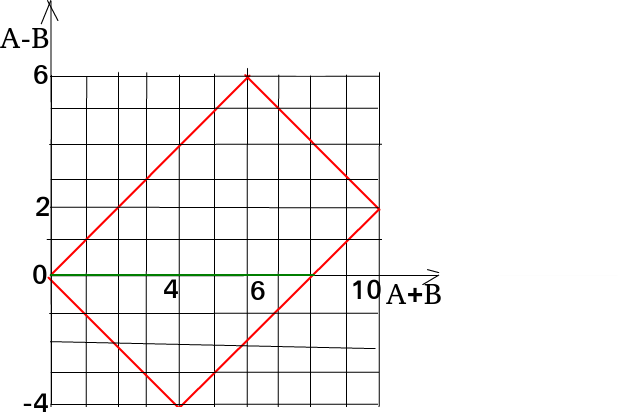
\includegraphics[width=.4\textwidth]{./pictures/t1v2_3.png}
  \caption{Пути}
  \label{fig:23}
\end{figure}

Красным обозначены граничные пути, зелёным --- линия, которой нельзя касаться.
В начале выборов разница у каждого кандидата было 0 голосов, в конце у кандидата $A$ было 6 голосов, а у кандидата $B$ --- 4 голоса.
Поэтому разность голосов в конце составляет 2 голоса.
Перевернём изображение (рис. \ref{fig:231}).

\begin{figure}[h!]
  \centering
  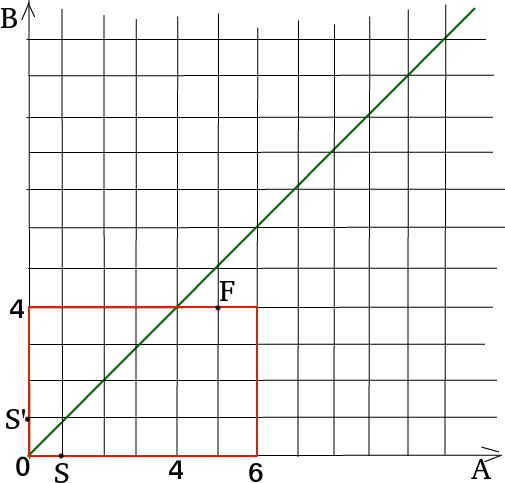
\includegraphics[width=.4\textwidth]{./pictures/t1v2_31.png}
  \caption{Метод отражений}
  \label{fig:231}
\end{figure}

Всего возможных путей есть столько, сколько путей из точки $S$ в точку $F$.
Их
$$ \left| \Omega \right| =
C_{6+4}^4 =
C_{10}^4 =
\frac{10!}{4! \cdot 6!} =
210.$$

Путей из точки $S$ в точку $F$ существует
$$ \left| S \rightarrow F \right| =
C_{5+4}^4 =
C_9^4 =
\frac{9!}{4! \cdot 5!} =
\frac{6 \cdot 7 \cdot 8 \cdot 9}{2 \cdot 3 \cdot 4} =
\frac{6 \cdot 7 \cdot 9}{2} =
2 \cdot 7 \cdot 9 =
149.$$
Путей, которые касаются диагонали ---
$$ \left| S' \rightarrow F \right| =
C_{5+3}^3 =
C_8^3 =
\frac{8!}{3! \cdot 5!} =
\frac{6 \cdot 7 \cdot 8}{2 \cdot 3} =
7 \cdot 8 =
56.$$

Тогда путей,
которые не пересекают диагональ и удовлетворяют указанному в условии событию $C$ будет
$ \left| C \right| =
\left| S \rightarrow F \right| - \left| S' \rightarrow F \right| =
189 - 56 =
133$.
И его вероятность равна
$$P \left( C \right) =
\frac{ \left| C \right| }{ \left| \Omega \right| } =
\frac{183}{210}.$$

\subsubsection*{4}

\textit{Задание.} На отрезок наугад брошено две точки.
Найдите вероятность того, что из трёх образованных отрезков можно составить треугольник.

\textit{Решение.} Пусть отрезок начинается в точке 0 и заканчивается в точке $c$.
Выбираем на нём наугад две точки: точку $a$ и точку $b$, причём $a$ лежит не правее $b$ (рис. \ref{fig:24}).

\begin{figure}[h!]
  \centering
  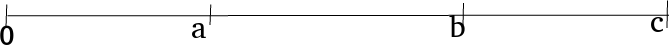
\includegraphics[width=.4\textwidth]{./pictures/t1v2_4.png}
  \caption{Отрезок $ \left[ 0, c \right] $}
  \label{fig:24}
\end{figure}

Тогда пространство элементарных исходов имеет вид $ \Omega =  \\
= \left\{ \left( a, b \right): 0 \leq a \leq b \leq c \right\} $.
Изобразив его на плоскости, видим, что это прямоугольный треугольник с катетами длиной $c$ (рис. \ref{fig:241}).

\begin{figure}[h!]
  \centering
  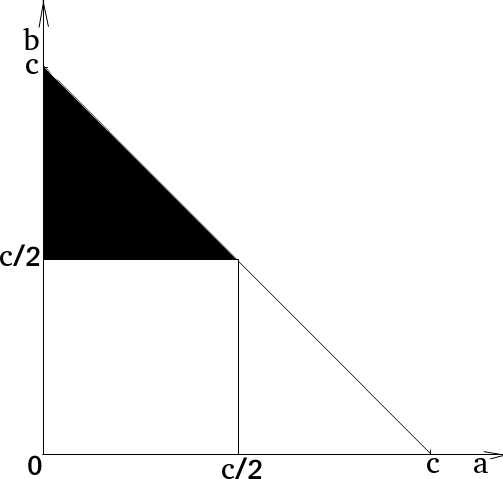
\includegraphics[width=.4\textwidth]{./pictures/t1v2_41.png}
  \caption{Пространство элементарных событий $ \Omega$ и событие $A$}
  \label{fig:241}
\end{figure}

Площадь треугольника равна
$$S_{ \Omega } =
\frac{1}{2} \cdot c \cdot c =
\frac{c^2}{2}.$$

Событие
$$A = \left\{ \left( a, b \right) \in \Omega: a \leq \frac{c}{2}, b \geq \frac{c}{2}, a \leq \frac{c}{2} + b \right\}.$$
Точки множества $A$ образуют прямоугольный треугольник с катетами $c/2$.
Его площадь равна
$$S_A =
\frac{1}{2} \cdot \frac{c}{2} \cdot \frac{c}{2} =
\frac{c^2}{8}.$$

Тогда вероятность события $A$ равна
$$P \left( A \right) =
\frac{S_A}{S_{ \Omega }} =
\frac{c^2}{8} \cdot \frac{2}{c^2} =
\frac{1}{4}.$$

\subsubsection*{5}

\textit{Задание.} В первой урне находятся 3 чёрных и 3 белых шарика, а во второй --- 2 чёрных и 3 белых шарика.
Из второй урны наугад вынули два шарика и переложили в первую.
После этого из первой урны вынимают два шарика.
Найдите вероятность того, что они окажутся разного цвета.

\textit{Решение.} Введём событие $A =$ \{вынутые после перекладывания шарики из первой урны окажутся разного цвета\}.
Введём гипотезы по поводу того,
каких цветов оказались шарики,
переложенные в первую урну из второй: $H_1 =$ \{чёрный, белый\}, $H_2 =$ \{белый, чёрный\}, $H_3 =$ \{чёрный, чёрный\}, $H_4 =$ \{белый, белый\}.
Найдём вероятности этих гипотез:
$$P \left( H_1 \right) =
\frac{2}{5} \cdot \frac{3}{4}, \,
P \left( H_2 \right) =
\frac{3}{5} \cdot \frac{2}{4}, \,
P \left( H_3 \right) =
\frac{2}{5}, \,
P \left( H_4 \right) =
\frac{3}{5}.$$

Найдём условные вероятности события $A$ при условии выполнения каждой из этих гипотез.
Пусть произошла гипотеза $H_1$.
Тогда в первой урне стало 4 чёрных и 4 белых шарика.
Вероятность того, что 2 вынутые шарика окажутся разного цвета, равна
$$P \left( \left. A \right| H_1 \right) =
\frac{4}{8} \cdot \frac{4}{7} \cdot 2.$$
Пусть произошла гипотеза $H_2$.
Тогда в первой урне стало 4 чёрных и 4 белых шарика.
Вероятность того, что 2 вынутые шарика окажутся разного цвета, равна
$$P \left( \left. A \right| H_2 \right) =
\frac{4}{8} \cdot \frac{4}{7} \cdot 2.$$
Пусть произошла гипотеза $H_3$.
Тогда в первой урне стало 5 чёрных и 3 белых шарика.
Вероятность того, что 2 вынутые шарика окажутся разного цвета, равна
$$P \left( \left. A \right| H_3 \right) =
\frac{5}{8} \cdot \frac{3}{7} \cdot 2.$$
Пусть произошла гипотеза $H_4$.
Тогда в первой урне стало 3 чёрных и 5 белых шарика.
Вероятность того, что 2 вынутые шарика окажутся разного цвета, равна
$$P \left( \left. A \right| H_4 \right) =
\frac{3}{8} \cdot \frac{5}{7} \cdot 2.$$

По формуле для полной вероятности
\begin{equation*}
\begin{split}
P \left( A \right) =
\sum \limits_{i=1}^4 P \left( H_i \right) \cdot P \left( \left. A \right| H_i \right).
\end{split}
\end{equation*}

\addcontentsline{toc}{section}{Вариант 3}
\section*{Вариант 3}

\subsubsection*{1}

\textit{Задание.} Что вероятней: выиграть у равносильного противника 3 шахматных партии из 4 или 5 партий из 8?

\textit{Решение.} Найдём вероятность выиграть 3 шахматные партии из четырёх.
Пространство элементарных событий состоит из $ \left| \Omega_1 \right| = 2^4$ элементов,
так как каждую из четырёх партий можно выиграть или проиграть.
Введём событие $A =$ \{3 партии из четырёх будут удачными\}.
Нужно выбрать одну партию из четырёх, которая не будет удачной --- это $C_4^1 = \left| A \right| $.
Тогда вероятность этого события равна
$$P \left( A \right) =
\frac{ \left| A \right| }{ \left| \Omega_1 \right| } =
\frac{C_4^1}{2^4} =
\frac{4}{4^2} =
\frac{1}{4}.$$

Найдём вероятность выиграть 4 шахматные партии из восьми.
Пространство элементарных событий в данном случае состоит из $ \left| \Omega_2 \right| = 2^8$ элементов.
Пусть событие $B =$ \{5 партий из восьми закончатся победой\}.
Нужно выбрать 5 партий из восьми, которые закончатся победой --- это
$$ \left| B \right| =
C_8^5 =
\frac{8!}{5! \cdot 3!} =
\frac{6 \cdot 7 \cdot 8}{2 \cdot 3} =
7 \cdot 8.$$
Тогда вероятность этого события равна
$$P \left( B \right) =
\frac{ \left| B \right| }{ \left| \Omega \right| } =
\frac{7  \cdot 8}{2^8} =
\frac{7}{2^5} =
\frac{7}{32}.$$

Сравним две полученные вероятности.
Для этого первую умножим на 8:
$$ \frac{8}{8} \cdot \frac{1}{4} =
\frac{8}{32}.$$
Видим, что
$$ \frac{8}{32} > \frac{7}{32},$$
поэтому $P \left( A \right) > P \left( B \right) $.
Тогда вероятность выиграть 3 шахматные партии из четырёх больше, чем вероятность выиграть 5 партий из восьми.

\subsubsection*{2}

\textit{Задание.} В сундуке лежат 9 красных, 6 синих и 5 зелёных пуговиц.
Наугад вынули 2 пуговицы.
Найдите вероятность того, что пуговицы разного цвета, если известно, что среди них нет зелёных.

\textit{Решение.} Опишем событие $A =$ \{среди двух пуговиц нет зелёных\}.
Возможны варианты: (красная, красная), (синяя, синяя), (красная, синяя), (синяя, красная).
Вероятность того, что вытянем одну красную и одну синюю пуговицу, равна
$$ \frac{9}{20} \cdot \frac{6}{19}.$$
Вероятность того, что две пуговицы будут красными, равна
$$ \frac{9}{20} \cdot \frac{8}{19}.$$
Наконец, вероятность того, что две пуговицы будут синими, равна
$$ \frac{6}{20} \cdot \frac{5}{19}.$$
Тогда по правилу суммы имеем вероятность указанного события:
\begin{equation*}
\begin{split}
P \left( A \right) =
\frac{2 \cdot 9 \cdot 6}{20 \cdot 19} + \frac{9 \cdot 8}{20 \cdot 19} + \frac{6 \cdot 5}{20 \cdot 19} =
\frac{9 \cdot 6 + 9 \cdot 4 + 3 \cdot 5}{10 \cdot 19} =
\frac{54 + 36 + 15}{10 \cdot 19} = \\
= \frac{105}{10 \cdot 19} =
\frac{21}{2 \cdot 19}.
\end{split}
\end{equation*}

Введём событие $B =$ \{пуговицы оказались разного цвета\}.
Найдём пересечение двух событий: $A \cap B =$ \{пуговицы оказались разного цвета, и среди них нет зелёных\}.
Есть два варианта: (красный, синий), (синий, красный).
Вероятность этого пересечения равна
$$P \left( A \cap B \right) =
\frac{2 \cdot 9 \cdot 6}{20 \cdot 19} =
\frac{9 \cdot 6}{10 \cdot 19} =
\frac{9 \cdot 3}{5 \cdot 19}.$$

Тогда по формуле для условной вероятность получаем, что
$$P \left( \left. B \right| A \right) =
\frac{P \left( A \cap B \right) }{P \left( A \right) } =
\frac{9 \cdot 3}{5 \cdot 19} \cdot \frac{2 \cdot 19}{21} =
\frac{9 \cdot 2}{5 \cdot 7} =
\frac{18}{35}.$$

\subsubsection*{3}

\textit{Задание.} На отрезок наугад брошены две точки.
Найдите вероятность того, что левый из трёх образованных отрезков будет самым коротким.

\textit{Решение.} Пусть отрезок начинается в точке 0 и заканчивается в точке $c$.
Выбираем на нём наугад две точки: точку $a$ и точку $b$, причём $a$ лежит не правее $b$ (рис. \ref{fig:24}).

Тогда пространство элементарных исходов имеет вид $ \Omega =  \\
= \left\{ \left( a, b \right): 0 \leq a \leq b \leq c \right\} $.
Изобразив его на плоскости, видим, что это прямоугольный треугольник с катетами длиной $c$ (рис. \ref{fig:33}).

\begin{figure}[h!]
  \centering
  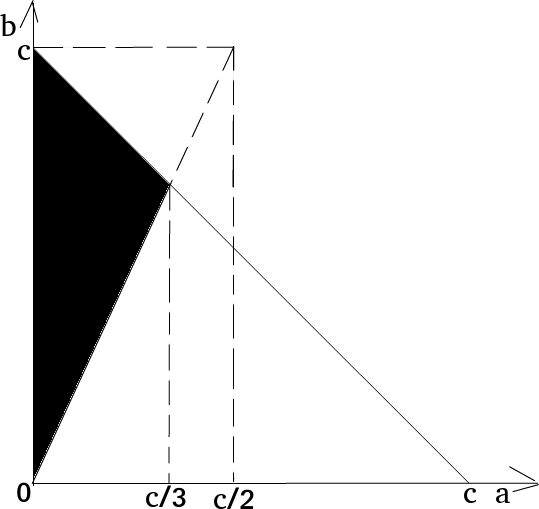
\includegraphics[width=.4\textwidth]{./pictures/t1v3_3.png}
  \caption{Пространство элементарных событий $ \Omega$ и событие $A$}
  \label{fig:33}
\end{figure}

Площадь треугольника равна
$$S_{ \Omega } =
\frac{1}{2} \cdot c \cdot c =
\frac{c^2}{2}.$$

Пусть событие $A = \left\{ \left( a, b \right) \in \Omega: a \leq b-a, a \leq c-b \right\} $.
Изобразив его на рисунке, видим, что это треугольник, образованный прямой $b = c - a$, прямой $b = 2a$ и одним из катетов исходного треугольника.
Его площадь найдём с помощью интеграла:
$$S_A =
\int \limits_0^{ \frac{c}{3} } \left( c - a \right) da =
\left. \left( ca - \frac{a^2}{2} \right) \right|_0^{ \frac{c}{3} } =
c \cdot \frac{c}{3} - \frac{c^2}{9 \cdot 2} =
\frac{c^2}{3} - \frac{c^2}{18} =
\frac{6c^2 - c^2}{18} =
\frac{5c^2}{18}.$$

Тогда вероятность этого события равна
$$P \left( A \right) =
\frac{S_A}{S_{ \Omega }} =
\frac{5c^2}{18} \cdot \frac{2}{c^2} =
\frac{5}{9}.$$

\subsubsection*{4}

\textit{Задание.} Частица совершает случайное симметрическое блуждание на прямой, делая шаг вправо или влево с вероятностью $1/2$.
Найдите вероятность того, что через $2n$ шагов частица впервые вернётся в исходную точку.

\textit{Решение.} Задача изображена на рисунке \ref{fig:34}.

\begin{figure}[h!]
  \centering
  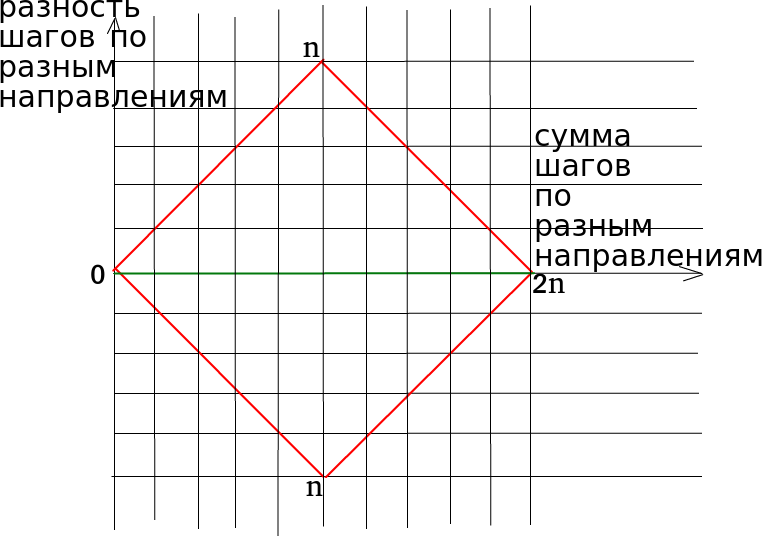
\includegraphics[width=.4\textwidth]{./pictures/t1v3_4.png}
  \caption{Задача про случайное блуждание частицы на прямой}
  \label{fig:34}
\end{figure}

Красным обозначены крайние пути, зелёным --- линия, которую нельзя пересекать.
Перевернём изображение (рис. \ref{fig:341}).

\begin{figure}[h!]
  \centering
  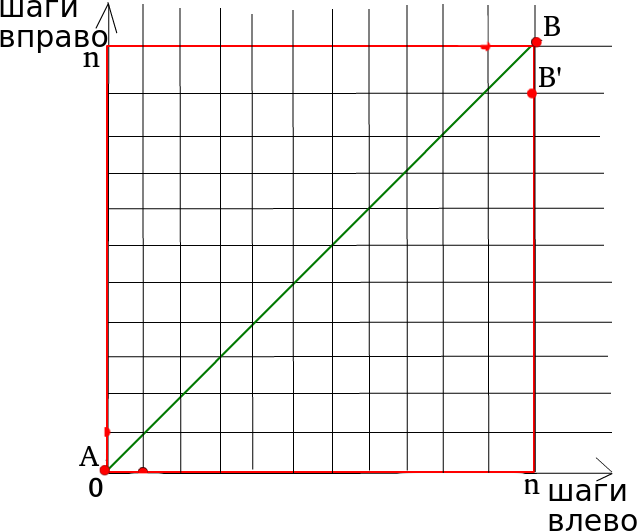
\includegraphics[width=.4\textwidth]{./pictures/t1v3_41.png}
  \caption{Метод отражений}
  \label{fig:341}
\end{figure}

Начальная точка --- точка $A$, конечная --- точка $B$.
Всего путей из $A$ в $B$ существует
$$ \left| A \rightarrow B \right| =
C_{n+n}^n =
C_{2n}^n =
\frac{ \left( 2n \right)!}{n!n!}.$$

Путей, которые пересекают диагональ будет
$$ \left| A' \rightarrow B \right| =
C_{n-1+n}^n =
C_{2n-1}^n =
\frac{ \left( 2n-1 \right)!}{n! \left( n-1 \right)!}.$$

Тогда путей, которые не пересекают диагональ будет
$$2 \left( \left| A \rightarrow B \right| - \left| A' \rightarrow B \right| \right) =
2 \cdot \left( \frac{ \left( 2n \right)!}{n!n!} - \frac{ \left( 2n-1 \right)!}{n! \left( n-1 \right)!} \right),$$
так как частица может двигаться и вправо, и влево.

Тогда вероятность указанного в условии задачи события равна
$$P =
\frac{2 \cdot \left( \frac{ \left( 2n \right)!}{n!n!} - \frac{ \left( 2n-1 \right)!}{n! \left( n-1 \right)!} \right) }{ \frac{ \left( 2n \right)!}{n!n!} }.$$

\subsubsection*{5}

\textit{Задание.}
Среди 5 стрелков есть 3 хороших, которые метко стреляют с вероятностью $0.8$, и 2 средних, которые попадают в цель с вероятностью $0.5$.
Вызвали наугад двух стрелков, они выстрелили по мишени и оба попали.
Найдите вероятность того, что стреляли два средних стрелка.

\textit{Решение.}
Введём событие $A =$ \{два стрелка попали по мишени\} и гипотезы о том,
каких стрелков вызвали: $H_1 =$ \{оба стрелка были хорошими\},
$H_2 =$ \{оба стрелка были средними\}, $H_3 =$ \{первый стрелок был хорошим, а второй --- средним\}, $H_4 =$ \{первый стрелок был средним, а второй хорошим\}.
Нужно найти вероятность
$$P \left( \left. H_2 \right| A \right) =
\frac{P \left( \left. A \right| H_2 \right) P \left( H_2 \right) }{ \sum \limits_{i=1}^4 P \left( \left. A \right| H_i \right) P \left( H_i \right) }.$$

Вероятность того, что выбрали два хороших стрелка равна
$$P \left( H_1 \right) =
\frac{3}{5} \cdot \frac{2}{4} =
\frac{3}{5} \cdot \frac{1}{2} =
\frac{3}{10}.$$

Вероятность того, что выбрали два средних стрелка равна
$$P \left( H_2 \right) =
\frac{2}{5} \cdot \frac{1}{4} =
\frac{1}{5 \cdot 2} =
\frac{1}{10}.$$

Вероятность того, что один из стрелков был хорошим, а второй --- средним равна
$$P \left( H_3 \right) =
P \left( H_4 \right) =
\frac{3}{5} \cdot \frac{2}{4} =
\frac{3}{10}.$$

Найдём условные вероятности:
\begin{equation*}
\begin{split}
P \left( \left. A \right| H_1 \right) =
\frac{8}{10} \cdot \frac{8}{10} =
\frac{4}{5} \cdot \frac{4}{5} =
\frac{16}{25}, \,
P \left( \left. A \right| H_2 \right) =
\frac{1}{2} \cdot \frac{1}{2} =
\frac{1}{4}, \,
P \left( \left. A \right| H_3 \right) = \\
= P \left( \left. A \right| H_4 \right) =
\frac{8}{10} \cdot \frac{1}{2} =
\frac{4}{5 \cdot 2} =
\frac{2}{5}.
\end{split}
\end{equation*}

Тогда по формуле Байеса получаем
$$P \left( \left. H_2 \right| A \right) =
\frac{ \frac{1}{4} \cdot \frac{1}{10} }{ \frac{3}{10} \cdot \frac{16}{25} + \frac{1}{4} \cdot \frac{1}{10} + 2 \cdot \frac{3}{10} \cdot \frac{2}{5} }$$
